\documentclass[dvipdfmx]{beamer}

\AtBeginDvi{\special{pdf:tounicode 90ms-RKSJ-UCS2}} % 栞の文字化けを制御(日本語の場合必須)
\setbeamertemplate{navigation symbols}{} %ナビゲーションバーを消す


%%% 以下3つはハンドアウト印刷用
%\documentclass[dvipdfm,handout]{beamer}
%\usepackage{pgfpages}
\usepackage{comment}
\usepackage{amsmath}
\usepackage{algorithm}
\usepackage{algorithmic}
%\pgfpagesuselayout{4 on 1}[border shrink=3mm]


% 付録をページ番号に含めないためのコマンド
\newcommand{\backupbegin}{
\newcounter{framenumberappendix}
\setcounter{framenumberappendix}{\value{framenumber}}
}
\newcommand{\backupend}{
\addtocounter{framenumberappendix}{-\value{framenumber}}
\addtocounter{framenumber}{\value{framenumberappendix}}
}

%%% メインテーマ
%\usetheme{Berkeley}
%\usetheme{CambridgeUS}
%\usetheme{Default}
%\usetheme{Darmstadt}
%\usetheme{Hannover}
%\usetheme{lankton-keynote}
%\usetheme{Luebeck}
%\usetheme{Marburg}
\usetheme{Madrid}
%\usetheme{boxes}
%\usetheme{Bergen}
%\usetheme{Boadilla}
%\usetheme{Pittsburgh}
%\usetheme{Rochester}

\useinnertheme{rectangles}

%\useoutertheme{default}

%%% カラーテーマ(省略可)
\useoutertheme{infolines}
\usecolortheme[RGB={64,64,64}]{structure}     
%\definecolor{babyblue}{rgb}{0.54,0.81,0.94}                                                                                                
%\usecolortheme{dolphin}
%\usecolortheme{beaver}
%\usecolortheme{beetle}
\usecolortheme{crane}
%\usecolortheme{dolphin}
%\usecolortheme{seagull}
%\usecolortheme{wolverine}
%\usecolortheme{spruce}
%\usecolortheme{rose}
%\usecolortheme{seahorse}

%%% フォント
\renewcommand{\kanjifamilydefault}{\gtdefault} % 日本語フォントをゴシック
\usefonttheme[onlymath]{serif}
\usefonttheme[onlylarge]{structurebold}
%\usefonttheme{professionalfonts}
\fontencoding{\encodingdefault}
\fontfamily{\kanjifamilydefault}
\fontseries{\seriesdefault}
\fontshape{\shapedefault}
\selectfont
%\mathversion{bold} % 数式フォントをbold体

%%% インナー, アウターテーマ(省略可)
%\useinnertheme{circles}
%\useoutertheme{infolines}

%\logo{\includegraphics[width=1.5cm, height=1.5cm]{.jpg}} % ロゴをいれる
\setbeamertemplate{navigation symbols}{} % ナビゲーションバーなし
%\setbeamertemplate{background}[grid][step=5mm] % 背景グリッド
\setbeamertemplate{footline}[frame number] % ページ番号の表示
\setbeamerfont{footline}{size=\small,series=\bfseries}
\setbeamercolor{footline}{fg=black,bg=black}
\setbeamertemplate{caption}[numbered] % 図表番号の表示
%\setbeamerfont*{frametitle}{size=\normalsize,series=\bfseries} % フレーム文字の大きさ
\setbeamerfont*{frametitle}{size=\large,series=\bfseries} % フレームごとのフォントを設定変更できる。
\setbeamertemplate{frametitle}[default][center] % タイトルを中央寄せに設定変更できる。

\definecolor {mycolor1} {rgb} {0.00, 0.39, 0.00}
\definecolor {mycolor2} {rgb} {0.55, 0.27, 0.07}
\definecolor {mycolor3} {rgb} {0.63, 0.13, 0.94}

\definecolor {mycolorTitle} {rgb} {0.85, 0.855, 0.85}
\definecolor {mycolorHeader} {rgb} {0.93, 0.935, 0.93}

%ヘッダーとタイトルの色(fgで文字の色変えられる)
\setbeamercolor{frametitle}{bg = mycolorHeader}
\setbeamercolor{title}{bg = mycolorTitle}

\def\conpage{7}

%%% パッケージ
\usepackage[japanese]{babel}
\usepackage{inputenc}
\usepackage{times}
\usepackage{amsmath}
\usepackage{amssymb}
\usepackage{amsfonts}
\usepackage[T1]{fontenc}
\usepackage{hyperref}
\usepackage{algorithm,algorithmic}
\usepackage{ascmac}

%\usepackage{txfonts}
\usepackage{color}
%\usepackage{algpseudocode,algorithm}
%\usepackage{tikz}
%\usetikzlibrary{arrows}
%\tikzstyle{block}=[fill=blue,draw opacity=0.7,line width=1.4cm]

%\usepackage{listings,jlisting}
\usepackage{listings}

\lstset{%
  language={R},
  basicstyle={\small},%
  identifierstyle={\small},%
  commentstyle={\small\itshape},%
  keywordstyle={\small\bfseries},%
  ndkeywordstyle={\small},%
  stringstyle={\small\ttfamily},
  frame={tb},
  breaklines=true,
  columns=[l]{fullflexible},%
  numbers=left,%
  xrightmargin=0zw,%
  xleftmargin=3zw,%
  numberstyle={\scriptsize},%
  stepnumber=1,
  numbersep=1zw,%
  lineskip=-0.5ex%
}
%  \makeatletter
%    \renewcommand{\thealgorithm}{%
%    \thesection.\arabic{algorithm}}
%    \@addtoreset{algorithm}{section}
%  \makeatother

\newcommand{\bm}[1]{\mbox{\boldmath $#1$}}
\newcommand{\mapright}[1]{\mathop{\longrightarrow}\limits_{#1}}
\newcommand{\argmax}{\mathop{\rm argmax}\limits}

\renewcommand{\figurename}{図}
\renewcommand{\tablename}{表}

%%% Title, Author, etc.
\title[タイトル]{進捗報告 後期第1回}
%\subtitle[サブタイトル]{}
\author[発表者名]{塩濱研究室\\小坪琢人}
\institute[所属]{東京理科大学\ 工学部経営工学科4年\\学籍番号 4414036}
\date[日付]{2017年10月5日}

\begin{document}

\begin{frame}[plain]
\titlepage
\end{frame}
	
\begin{frame}{目次}
\tableofcontents
\end{frame}

\section{背景}
\begin{frame}{背景}

ベイジアンネットワークについて調べている中で, 因果推論というテーマに興味を持ちました.
機械学習や人工知能などかっこいい話はたくさんあるけれど, まず着目する事象の関係性を考えることが重要に思いました.

\end{frame}

\section{手法}
\begin{frame}{手法}

LiNGAM(Linear non-Gaussian Acyclic Models)と呼ばれる因果的構造モデル.

\end{frame}

\section{実験}
\begin{frame}[containsverbatim]{実験(1/2)}

$eps1, eps2$は外生変数と呼ばれ, ランダムに生成する. 外生変数をもとに$x1,x2$を順次決定する. この時$x2$を内生変数と呼ぶ.

\begin{lstlisting}[caption = LiNGAMの実行例1]
set.seed(4414)
n <- 500
# 外生変数
eps1 <- sign((rnorm(n))) * sqrt(abs(rnorm(n))) 
eps2 <- runif(n) - 0.5
# x1は内生変数
x2 <- 3 + eps2
x1 <- 0.9 * x2 + 7 + eps1
\end{lstlisting}

\end{frame}

\begin{frame}[containsverbatim]{実験(2/2)}

$eps1, eps2, eps3, eps4$は外生変数と呼ばれ, ランダムに生成する. 外生変数をもとに$x2,x1,x3,x4$を順次決定する. この時$x1,x2,x3$を内生変数と呼ぶ.

\begin{lstlisting}[caption = LiNGAMの実行例2]
set.seed(4414)
n <- 500 
eps1 <- sign(rnorm(n)) * sqrt(abs(rnorm(n))) 
eps2 <- runif(n) - 0.5 
eps3 <- sign(rnorm(n)) * abs(rnorm(n))^(1/3) 
eps4 <- rnorm(n)^2

x2 <- eps2 
x1 <- 0.9*x2 + eps1 
x3 <- 0.8*x2 + eps3 
x4 <- -x1 -0.9*x3 + eps4
\end{lstlisting}

\end{frame}

\section{結果}
\begin{frame}{結果}
実験1では$x2$が$x1$の関数であることを特定し, 実験2では$x1,x2,x3,x4$の因果関係を正しく判断することができた.
\end{frame}

\section{考察}
\begin{frame}{考察}
実験1において, 相関係数を調べると$0.245$となる.
相関はないのに, 因果関係を見抜いている??

\begin{figure}[H]
\begin{center}
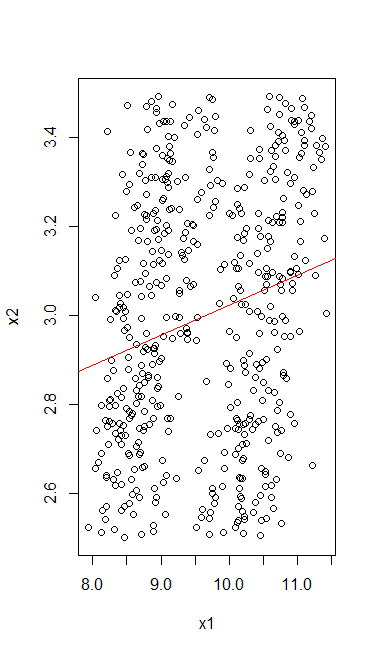
\includegraphics[clip,width=35mm]{data/sam1.png}
\caption{x1,x2の散布図, 回帰直線}
\end{center}
\end{figure}

\end{frame}

\section{今後の計画}
\begin{frame}{今後の計画}

VaRLiNGAMという時系列モデルに対して, 因果構造を発見するパッケージがあるのですがうまく動かないので調査します.

グラフィカルモデルの話しとかもう一回ちゃんと読み直します.

\end{frame}

\section{参考文献}
\begin{frame}[t,allowframebreaks, allowdisplaybreaks]{参考文献}

{\scriptsize
\begin{thebibliography}{99}
%\setlength{\itemsep}{-.5zw}
\beamertemplatetextbibitems

\bibitem{Shimizu}
清水昌平 (2017) 統計的因果探索. 講談社

\bibitem{Suzuki}
鈴木努 (2009) Rで学ぶネットワーク分析. 共立出版

%%\bibitem{Bishop}
%%C.M. Bishop (2007) パターン認識と機械学習 下. シュプリンガー・ジャパン

\end{thebibliography}
}

\end{frame}
\end{document}